\documentclass[12pt,letterpaper]{article}
\usepackage{apacite}
\usepackage[margin=0.8in]{geometry}
\linespread{1.3}

\usepackage{graphicx,textcomp}
\usepackage{setspace}
\usepackage{fullpage}
\usepackage{color}
\usepackage[reqno]{amsmath}
\usepackage{amsthm}
\usepackage{fancyvrb}
\usepackage{amssymb,enumerate}
\usepackage[all]{xy}
\usepackage{lscape}
\newtheorem{com}{Comment}
\usepackage{float}
\newtheorem{lem} {Lemma}
\newtheorem{prop}{Proposition}
\newtheorem{thm}{Theorem}
\newtheorem{defn}{Definition}
\newtheorem{cor}{Corollary}
\newtheorem{obs}{Observation}
\usepackage[compact]{titlesec}
\usepackage{dcolumn}
\usepackage{tikz}
\usetikzlibrary{arrows}
\usepackage{multirow}
\usepackage{xcolor}
\newcolumntype{.}{D{.}{.}{-1}}
\newcolumntype{d}[1]{D{.}{.}{#1}}
\definecolor{light-gray}{gray}{0.65}
\usepackage{url}

\usepackage{listings}
\usepackage{color}

\definecolor{codegreen}{rgb}{0,0.6,0}
\definecolor{codegray}{rgb}{0.5,0.5,0.5}
\definecolor{codepurple}{rgb}{0.58,0,0.82}
\definecolor{backcolour}{rgb}{0.95,0.95,0.92}

\lstdefinestyle{mystyle}{
	backgroundcolor=\color{backcolour},   
	commentstyle=\color{codegreen},
	keywordstyle=\color{magenta},
	numberstyle=\tiny\color{codegray},
	stringstyle=\color{codepurple},
	basicstyle=\footnotesize,
	breakatwhitespace=false,         
	breaklines=true,                 
	captionpos=b,                    
	keepspaces=true,                 
	numbers=left,                    
	numbersep=5pt,                  
	showspaces=false,                
	showstringspaces=false,
	showtabs=false,                  
	tabsize=2
}
\lstset{style=mystyle}
\newcommand{\Sref}[1]{Section~\ref{#1}}
\newtheorem{hyp}{Hypothesis}


\title{Dublin Bikes Report} 
\date{19/04/2023}
\author{Caitlín Cooney \& Jack Merriman}

\begin{document}
\maketitle

	\section{Introduction}
	
	\paragraph{}
	\noindent The two tasks chosen by our research team are:\\
	\textbf{1.} To assess the impact of the pandemic on the city-bike usage;\\
	\textbf{2.} To estimate how the city-bike usage would have been without the pandemic.\\
	
	\paragraph{Station Selection:}
	To decrease computational times we decided to focus on three bike stations. Rather than choose them arbitrarily, we used the \textit{k-means} clustering algorithm to divide Dublin's stations into $k = 3$ clusters based on latitude and longitude, then choose the nearest station with the largest possible capacity of $40$ stands to the centroid of each cluster. This ensures an unbiased selection of 3 stations representing various parts of Dublin's geography without any being on the periphery of the network.\\
	
	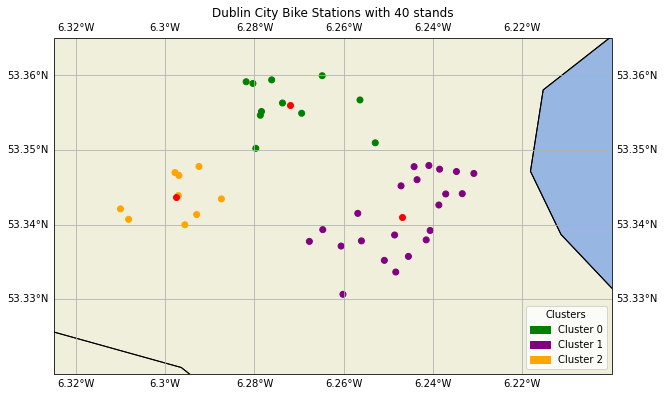
\includegraphics[width=\textwidth]{kmeans.png}
	
	
	
	
\end{document}
